\subsection{Tests Objekterkennung}
\label{sec_testObj}
Für diese Arbeit ist eine verlässliche Erkennung auf Simulationsbildern wichtig. Aus diesem Grund beziehen sich die Tests auf Simulationsbilder. Außerdem werden noch Tests auf Echtdaten durchgeführt, um das Verfahren zu evaluieren.\\
Für die Tests werden verschiedene Szenarien verwendet. Zunächst wird ein gerades Objekt, das komplett zu sehen ist, getestet [Abb. \ref{testStraightObj}]. Dieser Test repräsentiert das einfachste Szenario zur Detektion. Im zweiten Test wird dieses gerade Objekt vom Meeresboden verdeckt [Abb. \ref{testhalfObj}], um eine Detektion zu erschweren.\\
Im dritten Test wird ein Objekt betrachtet, das innerhalb des Bildes abgeknickt ist [Abb. \ref{testknickObj}]. Dabei wird getestet, wie sich die verschiedenen Ausrichtungen innerhalb eines Bildes auf die Detektion auswirken.
Ein vierter Test überprüft das Verhalten der Objekterkennung, wenn kein Objekt im Bild zu sehen ist. Hier sollte keine erfolgreiche Detektion entstehen. Alle Tests werden unter verschiedensten Sichtbedingungen durchgeführt. Die ursprünglichen Simulationsbilder als einfachsten Test, die Bildqualität, in der die meisten Testläufe des AUVs durchgeführt wurden und Bilder unter sehr schlechten Sichtbedingungen, in denen es schwer ist überhaupt ein Objekt zu entdecken.\\

Auf den nachfolgenden Seiten sind die Ergebnisse dieser Tests aufgeführt. Wie zu erwarten war, werden die Objekte und ihre Ausrichtungen im ursprünglichen Simulationsbild am besten erkannt. Hier sind die Grenzen zwischen Meeresboden und Objekt am klarsten und das Binärbild bildet das Objekt nahezu optimal ab. Ebenso kann der Templateschwellenwert so hoch gesetzt werden, dass keine Störpunkte vorhanden sind.\\
Die Tests mit schlechteren Sichtbedingungen führen ebenfalls zu guten Ergebnissen. In den Binärbildern sind oftmals \textit{wellenförmige} Kanten zu beobachten, die teilweise zu leicht fehlerhaften Detektionen der Ausrichtung führen. Zurückzuführen sind diese Kanten darauf, dass das Objekt aufgrund der Textur nicht überall gleich hohe Pixelwerte hat und so die \textit{dunkleren} Bereiche am Rand des Objektes den Schwellenwert nicht mehr überschreiten. Da der Unterschied zwischen Meeresboden und Objekt bei diesen Sichtbedingungen nicht so groß ist wie im ursprünglichen Bild, kann der Schwellenwert nicht weiter gesenkt werden, ohne zu viele Störpunkte zu erhalten.\\
Unter sehr schlechten Sichtbedingungen werden die Objekte noch immer gut detektiert. Jedoch sind in einigen Binärbildern trotz der einfachen Umgebung bereits viele Störpunkte sichtbar. Auch komplett ohne Objekt sind Punkte vorhanden. Ebenso wird das Objekt im Binärbild nicht mehr so gut abgebildet, wie unter besseren Bedingungen. Die bereits erwähnten \textit{wellenförmigen} Kanten sind auch hier zu beobachten.\\

\todo{b)s neu machen auf gleiche Größe}
\subsubsection*{Tests auf Simulationsbildern}
\begin{figure}[H]
\begin{tabular}{cc}
\subfloat[Objekt in ursprünglichem Simulationsbild]{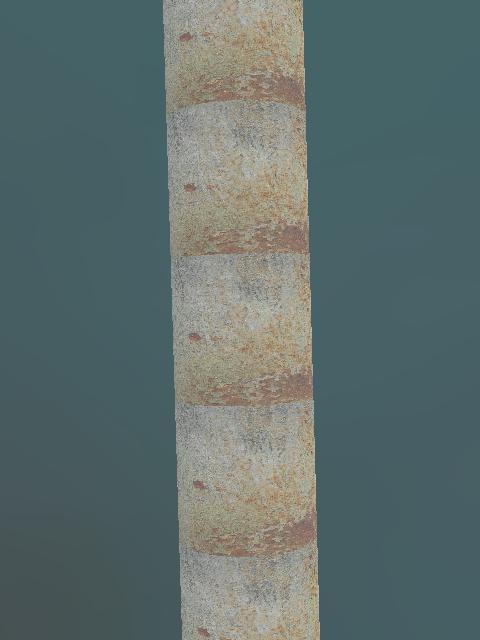
\includegraphics[width=0.5\textwidth,height=0.2\textheight]{/imageProcessing/gradeOptimal.jpg}}&
\subfloat[Detektiertes Objekt im ursprünglichen Simulationsbild]{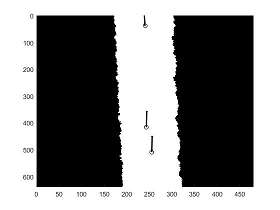
\includegraphics[width=0.5\textwidth,height=0.2\textheight]{/imageProcessing/gradeOptimalFin.jpg}}\\
\subfloat[Objekt unter schlechteren Sichtbedingungen]{
\includegraphics[width=0.5\textwidth,height=0.2\textheight]{/imageProcessing/gradeTestQuali.jpg}}&
\subfloat[Detektiertes Objekt unter schlechteren Sichtbedingungen]{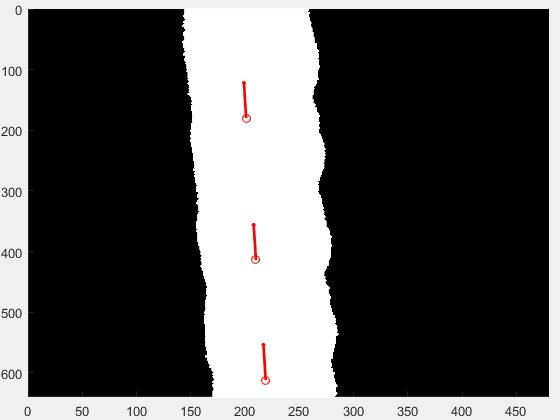
\includegraphics[width=0.5\textwidth,height=0.2\textheight]{/imageProcessing/gradeTestQualiFin.jpg}}\\
\subfloat[Objekt unter sehr schlechten Sichtbedingungen]{
\includegraphics[width=0.5\textwidth,height=0.2\textheight]{/imageProcessing/gradeschlecht.jpg}}&
\subfloat[Detektiertes Objekt unter sehr schlechten Sichtbedingungen]{\includegraphics[width=0.5\textwidth,height=0.2\textheight]{/imageProcessing/gradeschlechtfin.jpg}}
\end{tabular}
\caption{Ein gerades Objekt, dass ohne Einschränkungen zu sehen ist wird unter verschiedenen Sichtbedingungen und Bildqualität getestet. Die Gerade wird unter allen Bedingungen gut detektiert. In \textit{f)} ist zu sehen, dass unter sehr schlechten Sichtbedingungen ein \textit{gezackter} Kantenverlauf entsteht.}
\label{testStraightObj}
\end{figure}
\begin{figure}[H]
\begin{tabular}{cc}
\subfloat[Objekt in ursprünglichem Simulationsbild]{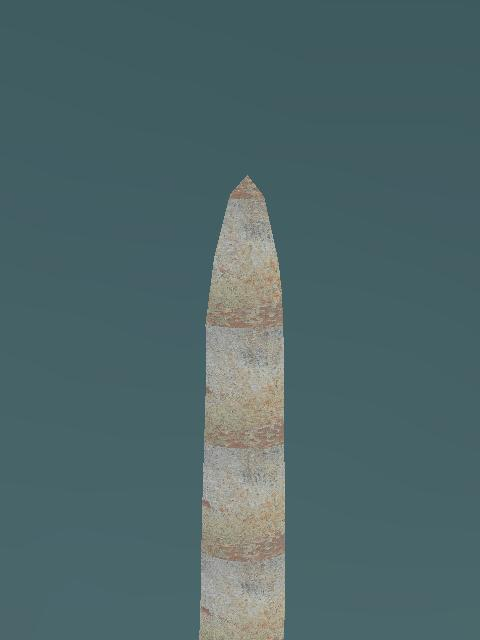
\includegraphics[width=0.5\textwidth,height=0.2\textheight]{/imageProcessing/gradeverborgen.jpg}}&
\subfloat[Detektiertes Objekt im ursprünglichen Simulationsbild]{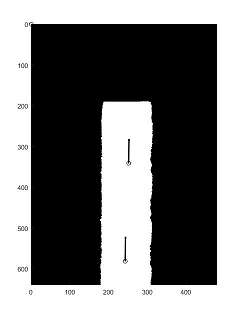
\includegraphics[width=0.5\textwidth,height=0.2\textheight]{/imageProcessing/gradeverborgenfin.jpg}}\\
\subfloat[Objekt unter schlechteren Sichtbedingungen]{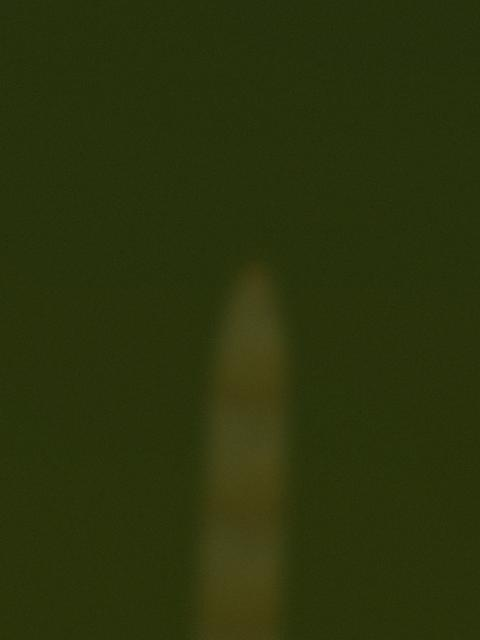
\includegraphics[width=0.5\textwidth,height=0.2\textheight]{/imageProcessing/gradeVerborgenTestQuali.jpg}}&
\subfloat[Detektiertes Objekt unter schlechteren Sichtbedingungen]{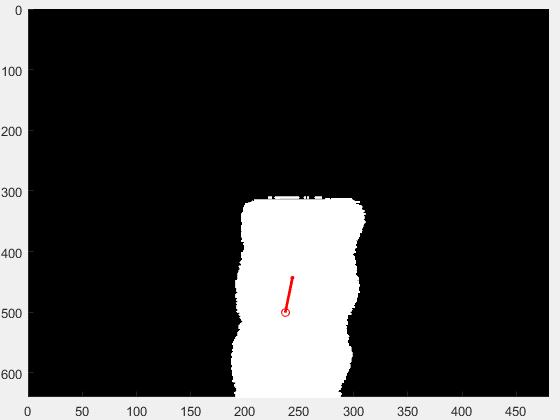
\includegraphics[width=0.5\textwidth,height=0.2\textheight]{/imageProcessing/gradeVerborgenTestQualiFin.jpg}}\\
\subfloat[Objekt unter sehr schlechten Sichtbedingungen]{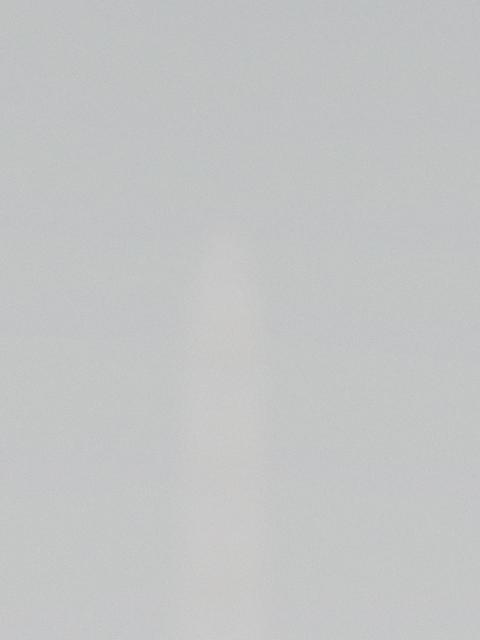
\includegraphics[width=0.5\textwidth,height=0.2\textheight]{/imageProcessing/gradeverborgenschlecht.jpg}}&
\subfloat[Detektiertes Objekt unter sehr schlechten Sichtbedingungen]{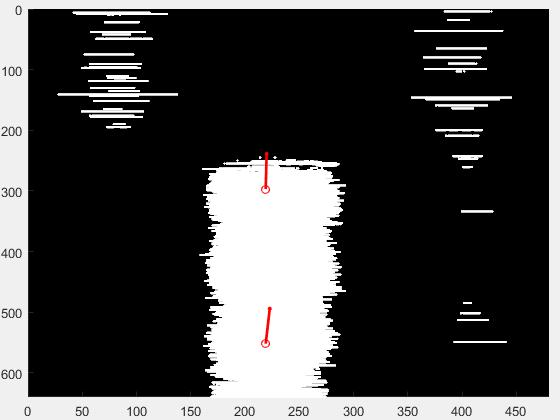
\includegraphics[width=0.5\textwidth,height=0.2\textheight]{/imageProcessing/gradeverborgenschlechtfin.jpg}}
\end{tabular}
\caption{Das verborgene Objekt wird unter allen Sichtbedingungen erkannt. Hier ist der Effekt der drei Segmente zu sehen. Während in \textit{b)} und \textit{f)} das Objekt noch in zwei Segmenten detektiert wurde, ist das Objekt in \textit{d)} zu kurz um im zweiten Segment noch detektiert zu werden.}
\label{testhalfObj}
\end{figure}
\begin{figure}[H]
\begin{tabular}{cc}
\subfloat[Objekt in ursprünglichem Simulationsbild]{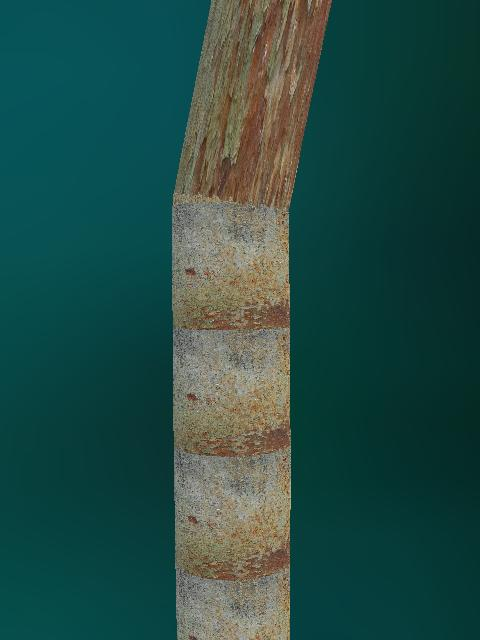
\includegraphics[width=0.5\textwidth,height=0.2\textheight]{/imageProcessing/knickOptimal.jpg}}&
\subfloat[Detektiertes Objekt im ursprünglichen Simulationsbild]{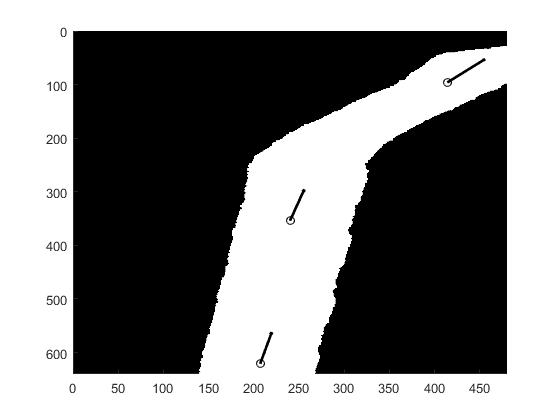
\includegraphics[width=0.5\textwidth,height=0.2\textheight]{/imageProcessing/knickoptimalfin.jpg}}\\
\subfloat[Objekt unter schlechteren Sichtbedingungen]{
\includegraphics[width=0.5\textwidth,height=0.2\textheight]{/imageProcessing/knickTestQuali.jpg}}&
\subfloat[Detektiertes Objekt unter schlechteren Sichtbedingungen]{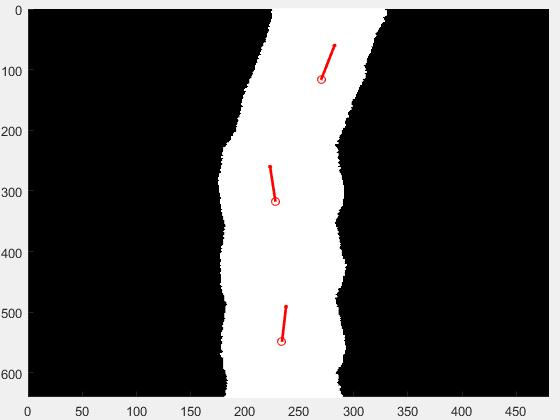
\includegraphics[width=0.5\textwidth,height=0.2\textheight]{/imageProcessing/knickTestQualiFin.jpg}}\\
\subfloat[Objekt unter sehr schlechten Sichtbedingungen]{\includegraphics[width=0.5\textwidth,height=0.2\textheight]{/imageProcessing/knickSchlecht.jpg}}&
\subfloat[Detektiertes Objekt unter sehr schlechten Sichtbedingungen]{\includegraphics[width=0.5\textwidth,height=0.2\textheight]{/imageProcessing/knickSchlechtFin.jpg}}
\end{tabular}
\caption{Das abgeknickte Objekt wird unter allen Sichtbedingungen erkannt. In \textit{d)} und \textit{f)} ist ein \textit{wellenförmiger} Kantenverlauf zu beobachten, der in \textit{d)} zu einer leicht falschen Bestimmung der Orientierung im geraden Bereich führt. In \textit{f)} ist zu sehen, dass die Störpixel im abgeknickten Bereich zu einer Fehldetektion der Orientierung führt.}
\label{testknickObj}
\end{figure}
\begin{figure}[H]
\begin{tabular}{cc}
\subfloat[Leeres ursprünglichem Simulationsbild]{
\includegraphics[width=0.5\textwidth,height=0.2\textheight]{/imageProcessing/nichts.jpg}}&
\subfloat[Keine Fehldetektion im ursprünglichen Simulationsbild]{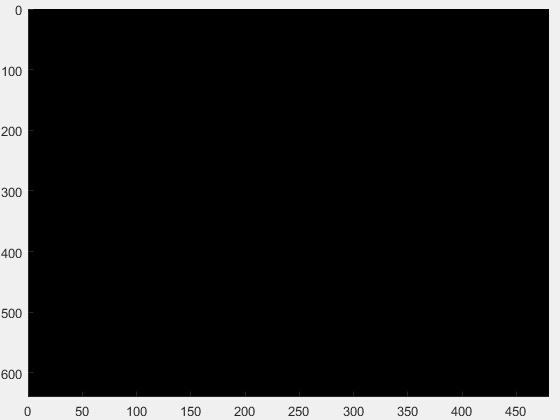
\includegraphics[width=0.5\textwidth,height=0.2\textheight]{/imageProcessing/nichtsoptimalfin.jpg}}\\
\subfloat[Leeres Bild unter schlechten Sichtbedingungen]{
\includegraphics[width=0.5\textwidth,height=0.2\textheight]{/imageProcessing/nichtsTestQuali.jpg}}&
\subfloat[Keine Fehldetektion unter schlechteren Sichtbedingungen]{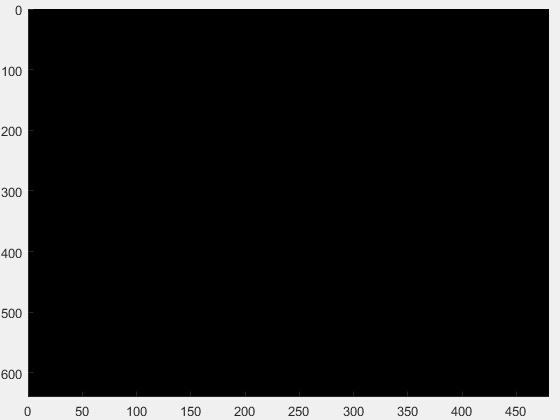
\includegraphics[width=0.5\textwidth,height=0.2\textheight]{/imageProcessing/nichtsTestQualiFin.jpg}}\\
\subfloat[Leeres Bild unter sehr schlechten Sichtbedingungen]{
\includegraphics[width=0.5\textwidth,height=0.2\textheight]{/imageProcessing/nichtsschlecht.jpg}}&
\subfloat[Einige Störpunkte aus dem Bild ohne Objekt unter sehr schlechten Sichtbedingungen]{\includegraphics[width=0.5\textwidth,height=0.2\textheight]{/imageProcessing/nichtsschlechtFin.jpg}}
\end{tabular}
\caption{In den Vergleichsbildern ohne Objekt wird auch unter allen Sichtbedingungen kein Objekt detektiert. Lediglich in \textit{f)} sind einige Störpunkte im Binärbild vorhanden, die auf den niedrig gewählten Templateschwellenwert [Kapitel \ref{sec_templ}] zurückzuführen sind.}
\label{testnothingObj}
\end{figure}

\subsubsection*{Tests auf Realbildern}
\label{realObjTests}
Um zu testen, ob das Verfahren auch bei echten Bildern funktioniert, wurden insgesamt 12 Bilder [Anhang \ref{anhang_objdecttests}] aus einem Testlauf des AUVs \textit{DAGON}\footnote{http://robotik.dfki-bremen.de/de/forschung/robotersysteme/dagon.html} während des Projektes \textit{CUSLAM}\footnote{http://robotik.dfki-bremen.de/de/forschung/projekte/cuslam.html} im Unisee getestet. Diese Testbilder wurden so ausgewählt, dass die relevanten Fälle abgedeckt sind. Es werden Bilder mit sehr schlechten Sichtbedingungen, in denen die Pipeline sehr schwer zu erkennen ist, in anderen ist die Pipeline sehr gut sichtbar und hebt sich deutlich vom Hintergrund ab. Zudem werden noch Bilder gewählt, in denen die Pipeline zuerst gut und im Bildverlauf immer schlechter sichtbar ist. Außerdem sind in der Auswahl noch Bilder, in denen die Pipeline direkt angestrahlt wird und dadurch sehr stark reflektiert.\\
In den Bildern, in denen die Pipeline kaum zu erkennen ist, wie in Abbildung \ref{rp_a} oder \ref{rp_b}, muss der Schwellenwert für das Template entsprechend niedrig gesetzt werden, was zu vielen Punkten im Binärbild führt, die nicht zum Objekt gehören. In Bildern, in denen die Pipeline direkt angestrahlt wird und klar heller ist als der Hintergrund, wie in Abbildung \ref{realData_good}, kann der Schwellenwert höher angesetzt werden, um weniger Störpunkte zu erhalten.

\begin{figure}[H]
\begin{tabular}{cc}
\subfloat[]{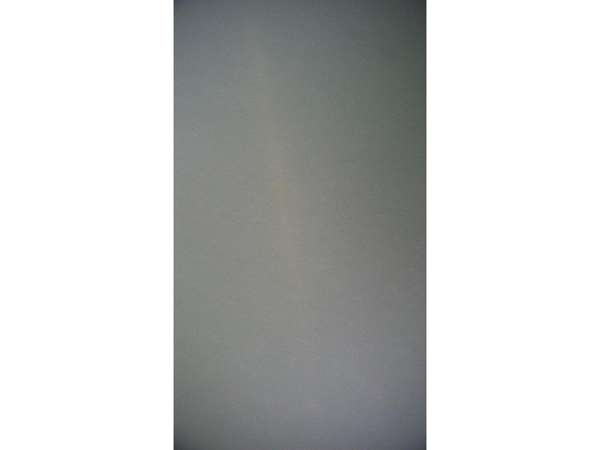
\includegraphics[height=0.2\textheight,width=0.5\textwidth]{imageProcessing/realPipe/001orgImstart.jpg}\label{rp_a}}&
\subfloat[]{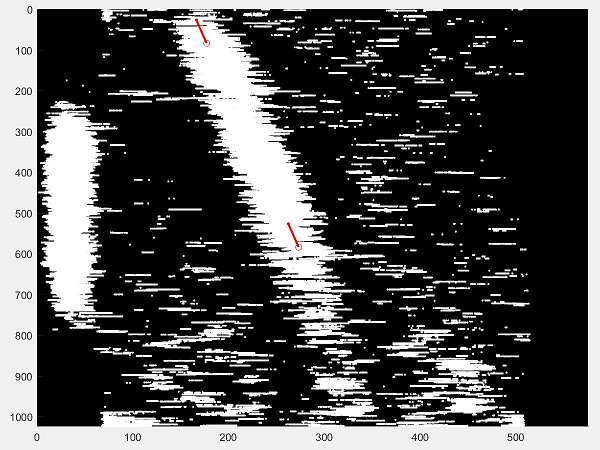
\includegraphics[height=0.2\textheight,width=0.5\textwidth]{imageProcessing/realPipe/001detectedImage.jpg}\label{rp_a}}\\
\subfloat[]{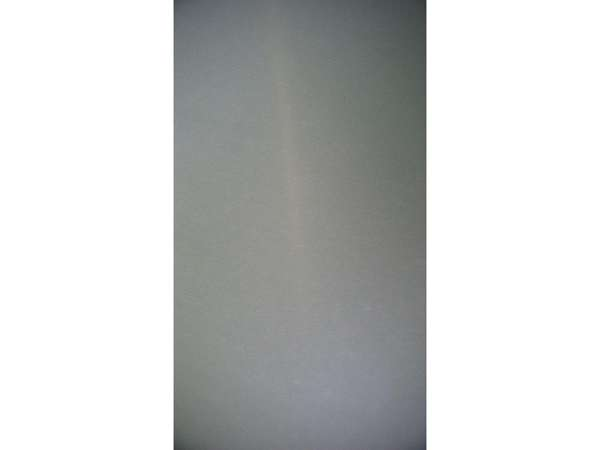
\includegraphics[height=0.2\textheight,width=0.5\textwidth]{imageProcessing/realPipe/002orgImstart.jpg}\label{rp_b}}&
\subfloat[]{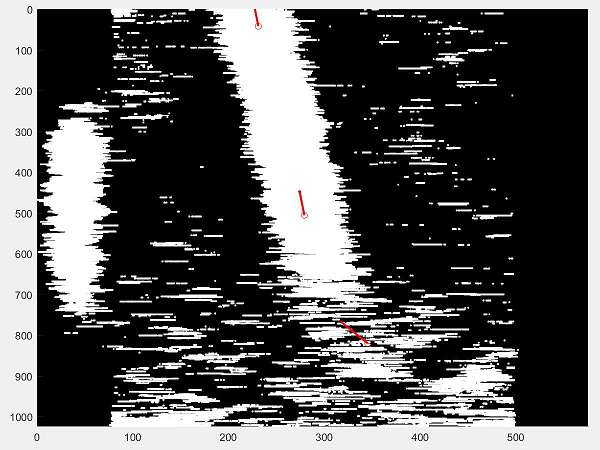
\includegraphics[height=0.2\textheight,width=0.5\textwidth]{imageProcessing/realPipe/002detectedImage.jpg}\label{rp_b}}
\end{tabular}
\caption{Tests der Objekterkennung auf realen Bildern aufgenommen im Unisee vom AUV \textit{DAGON}. Trotz sehr schlechter Sichtbedingungen und vieler Störpunkten im Binärbild wird die Pipeline in den oberen zwei Segmenten gut erkannt. In \textit{d)} ist im unteren Bereich eine Fehldetektion aufgrund der hohen Störpunktdichte in diesem Bereich. Die Randbereiche werden während des Binärisierungsprozess am Bild hinzugefügt, um das Template auch auf den ersten und letzten Pixeln anwenden zu können. Diese Bereiche werden bei der Detektion nicht betrachtet.}
\label{realData_bad}
\end{figure}

\begin{figure}[H]
\begin{tabular}{cc}
\subfloat[]{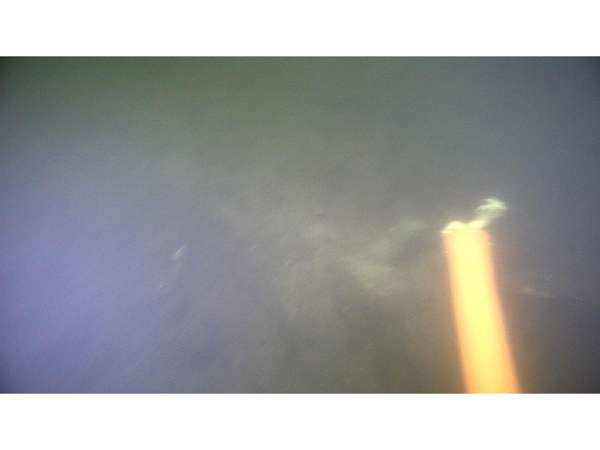
\includegraphics[height=0.2\textheight,width=0.5\textwidth]{imageProcessing/realPipe/008orgImstart.jpg}}&
\subfloat[]{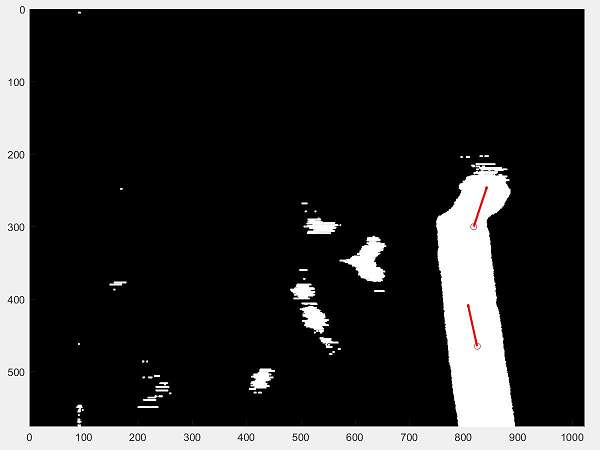
\includegraphics[height=0.2\textheight,width=0.5\textwidth]{imageProcessing/realPipe/008detectedImage.jpg}}\\
\end{tabular}
\caption{Test der Objekterkennung auf einem realen Bild aufgenommen im Unisee vom AUV \textit{DAGON}. Die Pipeline reflektiert sehr stark und hebt sich dadurch deutlich vom Hintergrund ab. Jedoch gibt es eine starke Reflexion nah an der Pipeline, was zu einer Fehldetektion im zweiten Segment führt.}
\label{realData_good}
\end{figure}

In den durchgeführten Tests wird deutlich, dass die Objekterkennung unter verschiedensten Sichtbedingungen gute Ergebnisse liefert. Die Sichtbedingungen haben dabei einen Einfluss auf die Binärisierung des Eingabebildes. Je schlechter die Sichtbedingungen sind, desto geringer muss der Templateschwellenwert gewählt werden. Der Schwellenwert ist jedoch ausschlaggebend für die Qualität der Abbildung vom Objekt im Binärbild. Umso geringer der Schwellenwert gewählt wird, umso mehr Störpunkte sind auch im Binärbild vorhanden (vgl. Abb. \ref{realData_bad} mit \ref{realData_good}). Bei schlechten Bedingungen muss der Schwellenwert jedoch gering gewählt werden, um das Objekt abbilden zu können (vgl. Kapitel \ref{sec_templ}). Somit steigt bei schlechteren Sichtbedingungen die Gefahr falsche Detektionen aufgrund von Störpunkten zu erhalten oder auch Objekte zu detektieren, wo keine vorhanden sind.\label{dangerLowTempl}